% Chapter 03 - Reaction Kinetics.tex
% Copyright (c) 2014 - 2016, zhiayang@gmail.com
% Licensed under the Apache License Version 2.0.

\pagebreak
\part{Reaction Kinetics}


	\section{Collision Theory}
		The collision theory of reaction is used to represent how individual molecules of reactants actually behave in a given reaction.
		It models reactions as collisions between molecules, and thus there are three conditions that must be satisfied:

		\begin{bulletlist}
			& A collision must occur
			& The collision must occur with the molecules in the correct orientation
			& The molecules must collide with sufficient speed to overcome the activation energy
		\end{bulletlist}

		Furthermore, the rate of a given reaction depends on the number of effective collisions in a given amount of time --- the
		\itl{effective collision frequency}.

		The importance of having the correct orientation can be seen in the electrophilic addition of \ch{HBr} to an alkene; the \deltap
		on the \ch{H} atom is attacked by the electron-rich π-bond, so naturally the \ch{HBr} molecule must be oriented such that the \ch{H}
		end is facing the alkene.

	% end section



	\section{Activation Energy}

		Activation energy represents the minimum amount of energy required before a reaction can take place --- this is usually manifested as
		the kinetic energy of colliding molecules of reactants, using the collision theory model of reaction. For most reactions, the activation
		energy is sufficiently high that the rate of reaction is not ridiculously fast, given that there are an enormous number of collisions
		between molecules at any given time.


		\pagebreak
		\subsection{Reaction Pathway Diagram}

			Activation energy is often represented in two ways; firstly, in the reaction pathway diagram as shown below. Note that even though
			the reaction is exothermic (it releases energy), it still requires a minimum amount of activation energy (\ea) to take place. On a side
			note, at the top of the energy ``peak'', a theoretical activated complex or transition state is formed; this cannot be isolated, and
			exists only for a tiny amount of time.


			\diagram[1.0]{
				\begin{endiagram}[scale=2.0,offset=1.5,x-label-text=reaction pathway,y-label-text=energy]
					\ENcurve[step=1.5]{2,4.5,0}

					\ShowNiveaus[shift=-1.0,length=2.0,niveau=N1-1]
					\ShowNiveaus[shift=1.0,length=2.0,niveau=N1-3]

					\ShowEa[label,label-side=left,label-pos=0.2]
					\ShowGain[label,offset=-40mm]

					\draw[above] (N1-1) ++ (1,0) node {\small \hspace{-40mm}reactants};
					\draw[above] (N1-3) ++ (1,0) node {\small products};

				\end{endiagram}
			}

		% end subsection


		\subsection{Maxwell-Boltzmann Distribution Curve}

			The other way that activation energy can be seen is through a Maxwell-Boltzmann distribution curve.

			\begin{center}
			\begin{tikzpicture}

				\def\kB{1.3806488e-23}% boltzmann constant
				\def\temperature{298}% room temperature
				\def\Beta{1/(\kB*\temperature)}
				\def\amu{1.660538921e-27}% atomar mass unit in kg
				\def\mass{0.9*\amu}

				\begin{axis}[
					axis lines		= left,
					domain			= 0:6000,
					xlabel			= \textbf{$E_{k}(x)$},
					ylabel			= \textbf{$N(x)$},
					xtick			= \empty,
					ytick			= \empty,
					axis line style	= very thick,
					x label style	= {at={(0.9,-0.01)}},
					y label style	= {at={(0,0.5)}},
					ymin			= 0,
					ymax			= 0.0004
				]

					\addplot[color = black, name path = fn, very thick]{
						sqrt(2/pi)*(\mass*\Beta)^(3/2)*x^2*exp(-.5*\mass*\Beta*x^2)
					};

					\path[name path global = xaxis] (axis cs: 0,0) -- (axis cs: 6000,0);
					\node at (axis cs: 4000,-0.0000325) {$E_{a}$};

					\addplot[color = red, fill = blue, fill opacity = 0.50] fill between[
						of				= fn and xaxis,
						soft clip		= { domain = 4000:6000 },
					];

					\path[name path global = dtd] (axis cs:4000,0) -- (axis cs:4000,0.00020);

					\draw[
						ultra thick, red, dashed,
						name intersections = {of = fn and dtd, name = k},
						name intersections = {of = xaxis and dtd, name = m}
					] (k-1) -- (m-1);

				\end{axis}

			\end{tikzpicture}
			\end{center}

			The shaded area represents the total number of molecules whose energy is greater than the activation energy, and can undergo a
			successful reaction. Note that the reactant molecules must still be oriented correctly for a successful reaction.

			Activation energy is independent of the enthalpy change of the reaction, and instead depends on the reactants themselves; it is always
			positive, because bonds are always broken first before new bonds are formed.

			\begin{bulletlist}

			& If reactants are similarly charged, \ea will be high --- the reverse is also true
			& If the bonds that need to be broken are strong, \ea will be high

			\end{bulletlist}

			Activation energy also affects the rate of a reaction; the lower the \ea, the larger the fraction of molecules that are at or above
			this energy. Hence, the frequency of effective collisions increase, and hence rate of reaction increases as well.

		% end subsection
	% end section


	\section{Rates of Reaction}

		The rate of a reaction is primarily determined by the rate of change of the concentrations of the reactants and products. That is,
		the faster the concentration of products increases, the faster the rate of reaction. Conversely, the faster the decrease of
		concentration of reactants, the faster the rate of reaction.

		\begin{center}
		\begin{tikzpicture}

			\begin{axis}[
				axis lines		= left,
				domain			= 0:10,
				xlabel			= \textbf{$time/s$},
				ylabel			= \textbf{$reactant$ $conc.$},
				axis line style	= very thick,
				height			= 80mm,
				enlarge y limits = 0.15
			]

				\addplot[color = black, name path = fn, very thick]{
					10 * e^(-0.25 * x)
				};

				\addplot[color = blue, very thick, restrict x to domain = 0:2]{
					-2.5 * x + 10
				};

				\addplot[color = red, very thick, restrict x to domain = 3:6]{
					-0.85 * x + 7.00
				};

				\node at (axis cs: 3,8) {initial rate};
				\node at (axis cs: 7,4) {instantaneous rate};

			\end{axis}

		\end{tikzpicture}
		\end{center}

		Thus, from a concentration-time graph, it is possible to determine the rate of a reaction through the measurement of the gradient.
		The initial rate of reaction is the gradient at $t = 0$, the rate of reaction at a given point in time is simply the gradient at that
		point, and the average rate of reaction is simply the rate of change of concentration across the graph.


		\pagebreak

		The rate equation outlines the relationship between the concentration of a given reactant and the actual rate of the reaction.
		All its components must be found experimentally, through a tedious process of actually conducting an experiment. It has this
		general form:

		\txtdiagram{
			\schemestart[0,1.0,thick]
				Rate = k[A]\sps{x}[B]\sps{y} ... [C]\sps{z}
			\schemestop
		}{\vspace{-2em}}

		R is the rate of the reaction (in \si{\molarConc\per\second}). k is the constant of proportionality
		(discussed below); \itl{[A]}, \itl{[B]} etc. are the concentrations of each reactant, and \itl{x}, \itl{y}, and
		\itl{z} are the orders of reaction with respect to that reactant.

		For single-direction equations (ie. not dynamic equilibrium reactions), the rate equation typically only contains the reactants, not
		the products. Also, the orders of reaction of each reactant are independent of the stoichiometric coefficients of those reactants in
		the actual equation. That is to say, an equation with ``\ch{4 CO2}'' does not mean that the order of reaction with respect to
		\ch{CO2} has to be 4. (it can be, but it's coincidental)



		\subsection{Order of Reaction}

			The order of a reaction with respect to a certain reactant determines the magnitude of the change in the rate of reaction when the
			concentration of that reactant is changed. Since the orders of the reaction are exponents, then it can be inferred that, the
			increase or decrease in the rate of reaction would be equal to the change in the concentration of a given reactant, to the power
			of its order.

			For instance, given this reaction and its rate equation:

			\txtdiagram{
				\schemestart[0,1.0,thick]
					\ch{2 NO \stG} + \ch{2 H2 \stG}
					\arrow
					\ch{N2 \stG} + \ch{2 H2O \stG}
				\schemestop
			}{Rate = k[\ch{NO}]\sps{2}[\ch{H2}]}

			When the concentration of \ch{H2} is doubled, the rate of the reaction will double. However, when [NO] is doubled, the rate of the
			reaction will increase by 4x. This also shows that the coefficients of the reactants in the chemical equation has nothing to do
			with the its order of reaction.

			Orders of reaction are not restricted to nonzero integers, of course; if the order of reaction of a reactant is negative, then when
			its concentration is increased, the rate of reaction will decrease; fractional orders also exist.

			If the order of reaction of a reactant is 0, it is usually omitted from the rate equation, as changing its concentration has no
			effect on the rate of the reaction.

			The overall order of a reaction is simply the sum of the individual orders of its reactants.


		% end subsection


		\subsection{Rate Constant}

			The rate constant \itl{k} is an amalgamation of two factors; the activation energy of the reaction and the temperature
			of the system.

			In the presence of catalysts (discussed later), the activation energy of the reaction will decrease. As the concentrations of the
			reactants are not affected, the increase in the rate of reaction is manifested in the increase of the rate constant. Similarly, a
			change in temperature will also affect the rate constant, and hence the rate of the reaction.

			Since the concentration of the reactants is represented in \si{\molarConc}, and the final rate of the reaction is
			represented with \si{\molarConc\per\second}, the rate constant must have appropriate units to ``balance'' the units
			of the rate equation. Competent humans should be able to determine the units of the rate constant by comparing the appropriate powers.


		% end subsection

	% end section





	\pagebreak
	\section{Determination of Reaction Order}

		\subsection{Initial Rates Method}

			A reactant’s order of reaction can be determined through the measurement of its initial rate, whilst changing the initial
			concentration of one or more reactants.

			Given the initial concentrations of all reactants and the initial rate (for two equations), a relationship between the rates can be
			determined. For example:

			\diagram[1.5]{
				\schemestart[0,1.0,thick]
					$\frac{R_{1}}{R_{2}} = \frac{k(0.03)^{x}(1.0)^{y}(0.5)^{z}}{k(0.01)^{x}(1.0)^{y}(0.5)^{z}}$
				\schemestop
			}{\vspace{-1.5em}}

			Given that the initial rates R\sbs{1} and R\sbs{2} are known, basic math can be applied to solve for \itl{x}, \itl{y},
			or \itl{z}. (In this case, \itl{x})
		% end subsubsection


		\subsection{Large Excess Method}

			The other method of determining the order of a reaction would be to use all but one reactant in large excess. For the purposes of this
			method, large excess is defined as a concentration 10x or more than the usual. This means that the concentrations of the other
			reactants appear to be constant, making them pseudo-zero-order.

			The reaction must be carried out once per reactant; an aliquot of the reaction mixture is withdrawn, and the concentration of the
			reactant in question is measured, and plotted in a concentration-time graph. A few things are in order:

			\begin{bulletlist}
				&	The withdrawn aliquot must be quenched, either by using ice (cooling), or removing the catalyst if the reaction cannot proceed
					without it.

				&	The aliquot is usually titrated with something to determine its concentration.
			\end{bulletlist}

			The order of reaction can be determined by the shape of the graph (discussed below).


		% end subsubsection

	% end subsection




	\pagebreak
	\section{Rate Graphs}

		\subsection{Concentration-Time Graph}

			A concentration-time graph is arguably the most versatile and useful graph. In such graphs, the rate of the reaction is represented
			by the gradient of the graph. As such, the order of the reaction can be determined by the shape of the graph.

			Concentration-time graphs are often used with the ``large-excess'' method, so that only the concentration of the reactant being
			observed appears to change.


			\subsubsection{Zeroth Order Reactions}

				For the zero-order reaction graph below, the rate of the reaction, which is the gradient, is constant even as [E] decreases.
				Thus, the rate is unaffected by the concentration of [E], and thus is zero order with respect to [E].

				\begin{center}
				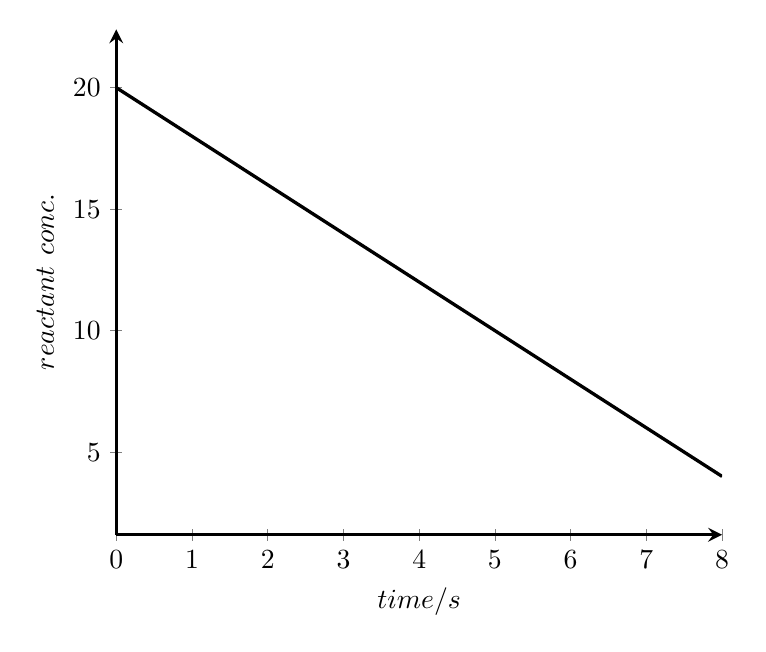
\begin{tikzpicture}

					\begin{axis}[
						axis lines		= left,
						domain			= 0:8,
						xlabel			= \textbf{$time/s$},
						ylabel			= \textbf{$reactant$ $conc.$},
						axis line style	= very thick,
						height			= 80mm,
						enlarge y limits = 0.15
					]

						\addplot[color = black, very thick]{
							-2.0 * x + 20
						};

					\end{axis}

				\end{tikzpicture}
				\end{center}

				The gradient of the graph is $-kt$, and the y-intercept is the initial concentration, [E]\sbs{0}.

			% end subsubsection




			\pagebreak
			\subsubsection{First Order Reactions}

				For first-order reactions, the concentration of the reactant decreases exponentially with time, and it has a constant half-life.
				This graph is a curve, because the rate of the reaction decreases as [A] decreases --- however, the rate of change of this
				decrease constant.


				\begin{center}
				\begin{tikzpicture}

					\begin{axis}[
						axis lines		= left,
						domain			= 0:1200,
						xlabel			= \textbf{$time/s$},
						ylabel			= \textbf{$reactant$ $conc.$},
						axis line style	= very thick,
						height			= 80mm,
						width			= 120mm,
						ytick			= {1, 0.5, 0.25, 0.125, 0},
						yticklabel style= {/pgf/number format/.cd,fixed zerofill,precision=3}
					]

						\addplot[color = black, very thick]{
							e^(-0.0025 * x)
						};


						\addplot[color = red, very thick, restrict x to domain = 0:280]{0.5};
						\addplot[color = red, very thick] coordinates {(280, 0) (280, 0.5)};

						\addplot[color = red, very thick, restrict x to domain = 0:560]{0.25};
						\addplot[color = red, very thick] coordinates {(560, 0) (560, 0.25)};

						\addplot[color = red, very thick, restrict x to domain = 0:840]{0.125};
						\addplot[color = red, very thick] coordinates {(840, 0) (840, 0.125)};

						\addplot[<->] coordinates {(0, 0.035) (280, 0.035)};
						\addplot[<->] coordinates {(280, 0.035) (560, 0.035)};
						\addplot[<->] coordinates {(560, 0.035) (840, 0.035)};

						\node at (axis cs: 140, 0.07) {$t_{\sfrac{1}{2}}$};
						\node at (axis cs: 420, 0.07) {$t_{\sfrac{1}{2}}$};
						\node at (axis cs: 700, 0.07) {$t_{\sfrac{1}{2}}$};

					\end{axis}

				\end{tikzpicture}
				\end{center}



				Above, $t_{\sfrac{1}{2}}$ represents the half-life. The half-life of a reaction is defined as the time taken for the concentration
				of a reactant to decrease to half its previous value. As it can be seen, in the graph above it goes from 0.10 to 0.05 to 0.025
				to 0.0125, and so on.

				Conversely, half-life can also be applied to the concentration of a product; it is the time taken for it to increase from 0 to 0.5,
				from 0.5 to 0.75, from 0.75 to 0.875, and so on. Note that the product concentration is just 1 - reactant concentration.


				\begin{center}
				\begin{tikzpicture}

					\begin{axis}[
						axis lines		= left,
						domain			= 0:1200,
						xlabel			= \textbf{$time/s$},
						ylabel			= \textbf{$product$ $conc.$},
						axis line style	= very thick,
						height			= 80mm,
						width			= 120mm,
						ytick			= {1, 0.875, 0.75, 0.5, 0},
						yticklabel style= {/pgf/number format/.cd,fixed zerofill,precision=3}
					]

						\addplot[color = black, very thick]{
							1 - e^(-0.0025 * x)
						};


						\addplot[color = red, very thick, restrict x to domain = 0:280]{0.5};
						\addplot[color = red, very thick] coordinates {(280, 0) (280, 0.5)};

						\addplot[color = red, very thick, restrict x to domain = 0:560]{0.75};
						\addplot[color = red, very thick] coordinates {(560, 0) (560, 0.75)};

						\addplot[color = red, very thick, restrict x to domain = 0:840]{0.875};
						\addplot[color = red, very thick] coordinates {(840, 0) (840, 0.875)};

						\addplot[<->] coordinates {(0, 0.035) (280, 0.035)};
						\addplot[<->] coordinates {(280, 0.035) (560, 0.035)};
						\addplot[<->] coordinates {(560, 0.035) (840, 0.035)};

						\node at (axis cs: 140, 0.07) {$t_{\sfrac{1}{2}}$};
						\node at (axis cs: 420, 0.07) {$t_{\sfrac{1}{2}}$};
						\node at (axis cs: 700, 0.07) {$t_{\sfrac{1}{2}}$};

					\end{axis}

				\end{tikzpicture}
				\end{center}


				For an overall first-order reaction, the half-life can be represented with this equation:

				\diagram[1.5]{
					\schemestart[0,1.0,thick]
						$t_{\sfrac{1}{2}} = \frac{ln(2)}{k}$
					\schemestop
				}{\vspace{-2em}}

				This means that the half-life is independent of the concentration of any reactant or product, and is only dependent on k,
				the rate constant.

			% end subsubsection




			\subsubsection{Second Order (and above) Reactions}

				The graph for second-order reactions has the same general exponential shape as the graph of a first-order reaction,
				except that the half-life is not constant. This is the key distinguishing difference between a first-order reaction and
				reactions of second-order and above.


				\begin{center}
				\begin{tikzpicture}

					\begin{axis}[
						axis lines		= left,
						domain			= 0:8000,
						xlabel			= \textbf{$time/s$},
						ylabel			= \textbf{$reactant$ $conc.$},
						axis line style	= very thick,
						height			= 80mm,
						width			= 120mm,
						ytick			= {1, 0.5, 0.25, 0.125, 0},
						yticklabel style= {/pgf/number format/.cd,fixed zerofill,precision=3}
					]

						\addplot[color = black, very thick]{
							e^(-0.0025 * x^0.8)
						};


						\addplot[color = red, very thick, restrict x to domain = 0:1]{0.5};
						\addplot[color = red, very thick] coordinates {(1130, 0) (1130, 0.5)};

						\addplot[color = red, very thick, restrict x to domain = 0:2]{0.25};
						\addplot[color = red, very thick] coordinates {(2660, 0) (2660, 0.25)};

						\addplot[color = red, very thick, restrict x to domain = 0:3]{0.125};
						\addplot[color = red, very thick] coordinates {(4460, 0) (4460, 0.125)};

						\addplot[color = red, very thick, restrict x to domain = 0:3]{0.0625};
						\addplot[color = red, very thick] coordinates {(6400, 0) (6400, 0.0625)};

						\addplot[<->] coordinates {(0.00, 0.035) (1130, 0.035)};
						\addplot[<->] coordinates {(1130, 0.035) (2660, 0.035)};
						\addplot[<->] coordinates {(2660, 0.035) (4460, 0.035)};
						\addplot[<->] coordinates {(4460, 0.035) (6400, 0.035)};

						\node at (axis cs: 765, 0.07) {$t_{\sfrac{1}{2}}$};
						\node at (axis cs: 1895, 0.07) {$t_{\sfrac{1}{2}}$};
						\node at (axis cs: 3560, 0.07) {$t_{\sfrac{1}{2}}$};
						\node at (axis cs: 5430, 0.07) {$t_{\sfrac{1}{2}}$};

					\end{axis}

				\end{tikzpicture}
				\end{center}

				Here, the half-life increases as the concentration of A decreases, so this is not a first- order reaction. It is possible to
				determine the precise order of a reaction using a rate- concentration graph (below) if the half-life is not constant.

			% end subsubsection

		% end subsubsection




		\pagebreak
		\subsection{Rate-Concentration Graph}

			The other useful graph is a plot of rate of reaction against concentration of a given reactant. This graph can be
			obtained in two ways;

			\begin{bulletlist}
				& Measure the gradient at intervals along the concentration-time graph (this is the rate), plotting these against the
				concentration of the reactant at that time

				& Measuring various initial rates of reaction from changing the initial concentration of a reactant, and plotting those.
				Note that all but the zero-order graphs pass through the origin, as rate is 0 when [A] is 0.
			\end{bulletlist}


			\subsubsection{Zeroth Order Reactions}

				If a reaction is zero-order with respect to a certain reactant, then the rate of reaction is independent of its concentration.
				Thus, since rate $= k[A]^{0}$, then rate $= k$, and the result is a horizontal line. The rate is constant at all values of [A].


				\begin{center}
				\begin{tikzpicture}

					\begin{axis}[
						axis lines		= left,
						domain			= 0:10,
						xlabel			= \textbf{[A]/\si{\molarConc}},
						ylabel			= \textbf{rate/\si{\molarConc\per\second}},
						axis line style	= very thick,
						height			= 80mm,
						width			= 120mm,
						xtick			= \empty,
						ytick			= \empty,
					]

						\addplot[color = black, very thick]{
							10
						};

					\end{axis}

				\end{tikzpicture}
				\end{center}


			% end subsubsection

			\pagebreak
			\subsubsection{First Order Reactions}

				For first-order reactions, the rate increases with the concentration of the reactant, in a linear manner.
				As such, rate $= k[A]$, which is in effect a $y = kx$ graph. Note that the graph must cut the origin, since the rate of
				reaction must be 0 when there is no reactant.

				\begin{center}
				\begin{tikzpicture}

					\begin{axis}[
						axis lines		= left,
						domain			= 0:10,
						xlabel			= \textbf{[A]/\si{\molarConc}},
						ylabel			= \textbf{rate/\si{\molarConc\per\second}},
						axis line style	= very thick,
						height			= 80mm,
						width			= 120mm,
						xtick			= \empty,
						ytick			= \empty,
						ymax			= 10,
						xmax			= 8
					]

						\addplot[color = black, very thick, restrict y to domain = 0:8]{
							1.2 * x
						};

					\end{axis}

				\end{tikzpicture}
				\end{center}

			% end subsubsection

			\subsubsection{Second Order (and above) Reactions}

				Of course, for reactions that are second-order or higher, the graph simply looks like an exponentially increasing curve.


				\begin{center}
				\begin{tikzpicture}

					\begin{axis}[
						axis lines		= left,
						domain			= 0:10,
						xlabel			= \textbf{[A]/\si{\molarConc}},
						ylabel			= \textbf{rate/\si{\molarConc\per\second}},
						axis line style	= very thick,
						height			= 80mm,
						width			= 100mm,
						xtick			= \empty,
						ytick			= \empty,
						ymax			= 10,
						xmax			= 8
					]

						\addplot[color = black, very thick, restrict y to domain = 0:8]{
							0.7 * x^2
						};

					\end{axis}

				\end{tikzpicture}
				\end{center}

				Of course, a better way to affirm the actual order of the reaction would be to plot a graph of rate against concentration
				squared --- resulting in a linear graph. A similar concept can be applied to the third order and above, plotting
				$[A]^{3}$ or $[A]^{4}$ or whatever.

			% end subsubsection

		% end subsection

	% end section





	\section{Factors Affecting Rate of Reaction}

		Note that all the factors below with the \itl{exception} of concentration and pressure reflect the change in the rate of reaction
		through a change in the rate constant, $k$.

		\subsection{Concentration and Pressure}

			When the concentration or pressure (for gas) of a reactant is increased, there are \itl{more molecules of reactant
			in a given volume}; thus, they are closer together, and they collide more frequently. Thus, there will be a
			\itl{greater frequency of effective collisions}, resulting in an increase in the rate of reaction.

			The statements above should be regurgitated to get the maximum marks. However, there is a caveat --- the effect on the rate of
			reaction is only applicable if the reactant in question appears in the rate equation. Hence, it must be in the rate-determining
			step as well.

		% end subsection

		\subsection{Surface Area of Solids}

			If the reaction involves a solid reactant, then the exposed surface area of the block is also a determining factor. With a
			greater surface area, there is a \itl{greater probability} that other reactants can come into contact with the solid, thus
			\itl{increasing the effective frequency of collisions}, thus increasing the rate of reaction.

			As an example, a single large block of solid reactant will result in a slower rate of reaction as opposed to the use of a
			finely powdered solid reactant. This effects a change in $k$.

		% end subsection


		\pagebreak
		\subsection{Temperature}

			Other than simply increasing the frequency of collisions, which the factors above have dealt with, a more effective method of
			increasing the rate of reaction is to increase the number of reactant molecules that are successful in colliding. There are two methods:

			\begin{bulletlist}
				& Increasing the average energy of the collisions
				& Reducing the energy barrier
			\end{bulletlist}

			By increasing the temperature, the rate constant $k$ is also increased. From the Maxwell-Boltzmann curve below, it can be seen that
			when the temperature of the system increases, there is a \itl{greater proportion} of molecules that have a kinetic energy greater
			than the activation energy; hence, more of the collisions that occur will result in a successful reaction.


			\begin{center}
			\begin{tikzpicture}

				\def\kB{1.3806488e-23}% boltzmann constant
				\def\to{300}% room temperature
				\def\tt{400}% room temperature
				\def\bo{1/(\kB*\to)}
				\def\bt{1/(\kB*\tt)}
				\def\amu{1.660538921e-27}% atomar mass unit in kg
				\def\mass{0.9*\amu}

				\begin{axis}[
					axis lines		= left,
					domain			= 0:6000,
					xlabel			= \textbf{$E_{k}(x)$},
					ylabel			= \textbf{$N(x)$},
					xtick			= \empty,
					ytick			= \empty,
					axis line style	= very thick,
					x label style	= {at={(0.9,-0.01)}},
					y label style	= {at={(0,0.5)}},
					ymin			= 0,
					ymax			= 0.0004
				]

					\addplot[color = black, name path = fn1, very thick]{
						sqrt(2/pi)*(\mass*\bo)^(3/2)*x^2*exp(-.5*\mass*\bo*x^2)
					};

					\addplot[color = black, name path = fn2, very thick]{
						sqrt(2/pi)*(\mass*\bt)^(3/2)*x^2*exp(-.5*\mass*\bt*x^2)
					};


					\path[name path global = xaxis] (axis cs: 0,0) -- (axis cs: 6000,0);
					\node at (axis cs: 4000,-0.0000325) {$E_{a}$};

					\addplot[color = red, fill = blue, fill opacity = 0.50] fill between[
						of				= fn2 and fn1,
						soft clip		= { domain = 4000:6000 },
					];

					\addplot[color = red, fill = green, fill opacity = 0.50] fill between[
						of				= fn1 and xaxis,
						soft clip		= { domain = 4000:6000 },
					];

					\node at (axis cs: 3000,0.00037) {300K};
					\node at (axis cs: 4000,0.00027) {400K};


					\path[name path global = dtd] (axis cs:4000,0) -- (axis cs:4000,0.00035);

					\draw[
						ultra thick, red, dashed,
						name intersections = {of = fn2 and dtd, name = k},
						name intersections = {of = xaxis and dtd, name = m}
					] (k-1) -- (m-1);

				\end{axis}

			\end{tikzpicture}
			\end{center}

			As the diagram illustrates, when the temperature is increased by 100K, the proportion of molecules that have a kinetic
			energy greater than the activation energy increases, from just the green area to the sum of the blue and green areas.

		% end subsection


		\subsection{Effect of Light}

			Light can also have an effect. When certain molecules absorb light energy, it is manifested as kinetic energy, resulting in a
			greater proportion of molecules that are beyond the energy barrier of the activation energy.

		% end subsection



		\pagebreak
		\subsection{Catalysts}

			The other method of course is to reduce the energy barrier itself. This is done by using a catalyst, which provides an
			\itl{alternative pathway} to the original. This is important --- it does not modify the activation energy of the actual
			reaction, it just provides another way to get to the products.

			From the Maxwell-Boltzmann curve, this would increase the number of molecules that have a kinetic energy greater
			than the activation energy, since this barrier is now lower.

			\begin{center}
			\begin{tikzpicture}

				\def\kB{1.3806488e-23}% boltzmann constant
				\def\temp{300}% room temperature
				\def\beta{1/(\kB*\temp)}
				\def\amu{1.660538921e-27}% atomar mass unit in kg
				\def\mass{0.9*\amu}

				\begin{axis}[
					axis lines		= left,
					domain			= 0:6000,
					xlabel			= \textbf{$E_{k}(x)$},
					ylabel			= \textbf{$N(x)$},
					xtick			= \empty,
					ytick			= \empty,
					axis line style	= very thick,
					x label style	= {at={(0.9,-0.01)}},
					y label style	= {at={(0,0.5)}},
					ymin			= 0,
					ymax			= 0.0004
				]

					\addplot[color = black, name path = fn, very thick]{
						sqrt(2/pi)*(\mass*\beta)^(3/2)*x^2*exp(-.5*\mass*\beta*x^2)
					};

					\path[name path global = xaxis] (axis cs: 0,0) -- (axis cs: 6000,0);

					\node at (axis cs: 3500,-0.0000325) {$E_{a_{2}}$};
					\node at (axis cs: 4000,-0.0000325) {$E_{a_{1}}$};


					\addplot[color = red, fill = green, fill opacity = 0.50] fill between[
						of				= fn1 and xaxis,
						soft clip		= { domain = 3500:4000 },
					];

					\addplot[color = red, fill = blue, fill opacity = 0.50] fill between[
						of				= fn1 and xaxis,
						soft clip		= { domain = 4000:6000 },
					];

					\path[name path global = dtd1] (axis cs:3500,0) -- (axis cs:3500,0.00035);

					\draw[
						ultra thick, red, dashed,
						name intersections = {of = fn and dtd1, name = k},
						name intersections = {of = xaxis and dtd1, name = m}
					] (k-1) -- (m-1);


					\path[name path global = dtd2] (axis cs:4000,0) -- (axis cs:4000,0.00035);

					\draw[
						ultra thick, red, dashed,
						name intersections = {of = fn and dtd2, name = k},
						name intersections = {of = xaxis and dtd2, name = m}
					] (k-1) -- (m-1);


				\end{axis}

			\end{tikzpicture}
			\end{center}

			The activation energy decreases from $E_{a_{1}}$ to $E_{a_{2}}$, so the number of molecules greater than the activation
			energy increases from just the blue area, to the sum of the blue and green areas.


			This effect can also be similarly illustrated with a reaction pathway diagram --- the one found on the cover page, you fool.

			\begin{center}
			\begin{endiagram}[scale=1.5,offset=1.5,x-label-text=,y-label-text=]
				\ENcurve[step=1.5]{0,4.5,2}
				\ENcurve[step=1.5,tikz={red,dotted}]{0,3,2}

				\ShowNiveaus[shift=-1.0,length=2.0,niveau=N1-1]
				\ShowNiveaus[shift=1.0,length=2.0,niveau=N1-3]

				\ShowEa[label,from={(N1-1) to (N1-2)}]
				\ShowGain[label]

				\draw[above] (N1-1) ++ (1,0) node {\small \hspace{-40mm}X};
				\draw[above] (N1-3) ++ (1,0) node {\small Y};

			\end{endiagram}
			\end{center}

			The red dotted line represents the alternative pathway that is taken. As such, the frequency of effective collisions increase,
			and thus rate of reaction increases.


		% end subsection

	% end section

% end part

























